\section{Another planetary defense mission: 2016 HO3}
\label{sec:7}

In this part we will look at the Asteroid HO3. We had to establish the thermophysical model of that asteroid.We have used the code used explain before and we have modified the differences value to fit with that asteroid.\newline

(469219) Kamo‘oalewa, provisionally designated 2016 HO3, is a quasi-satellite of the Earth3. It was discovered on April 27, 2016 by the Pan-STARRS program at the Haleakalā observatory on the Hawaiian island of Maui.\newline
He has an excentricity e = 0,10414290 , a period of revolution of 20 minutes.

The particularity of this asteroid is their speed, he have a rotation period of 20 minutes which is fast, to compare with the one we have study in this paper he is 36 times faster. Study that asteroid has permit to understand why the speed of rotation as an impact on the temperature.

To implement the map of this asteroid on Matlab we had to create a shapmodel of HO3, for that we have used SBMT and recreate the asteroid with the real dimension.\newline 

\begin{center}
    \captionsetup{type=figure}
    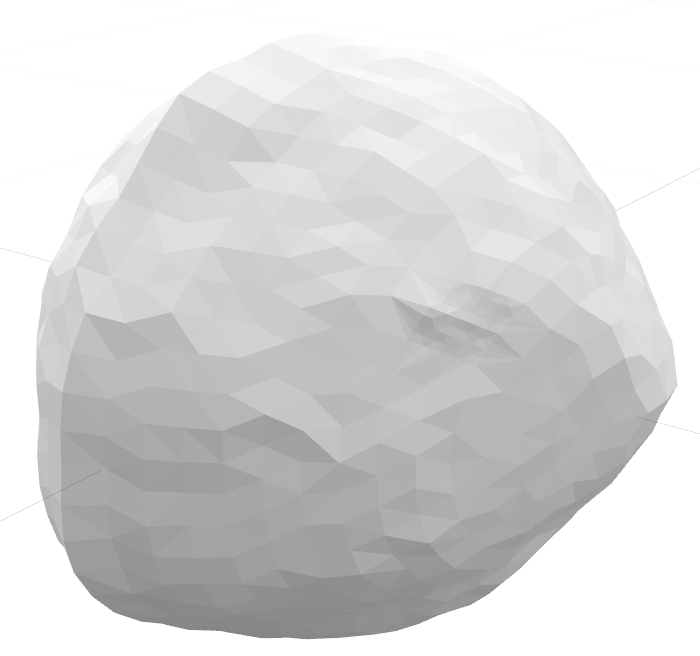
\includegraphics[scale=0.4]{rsc/HO3_shapemodel.png}
    \captionof{figure}{Shape model of HO3}
\end{center}

We have used a know asteroid already implement called Bennu and we have changed the size, Bennu had quite the same asperity than HO3 and gave us a better shape model for the temperature.


We have used the Matlab code see in the previous part to create the thermal map, we have take a $\Gamma$ = 500, A= 0.07, C= 0.25 and rho= 2146; .\\[10pt]

We have plot 2 map, one with 20 minutes speed and the other one with 12 hours, in the next 2 figures you will se the temperatures.\\[10pt]


\begin{center} % <-- added
    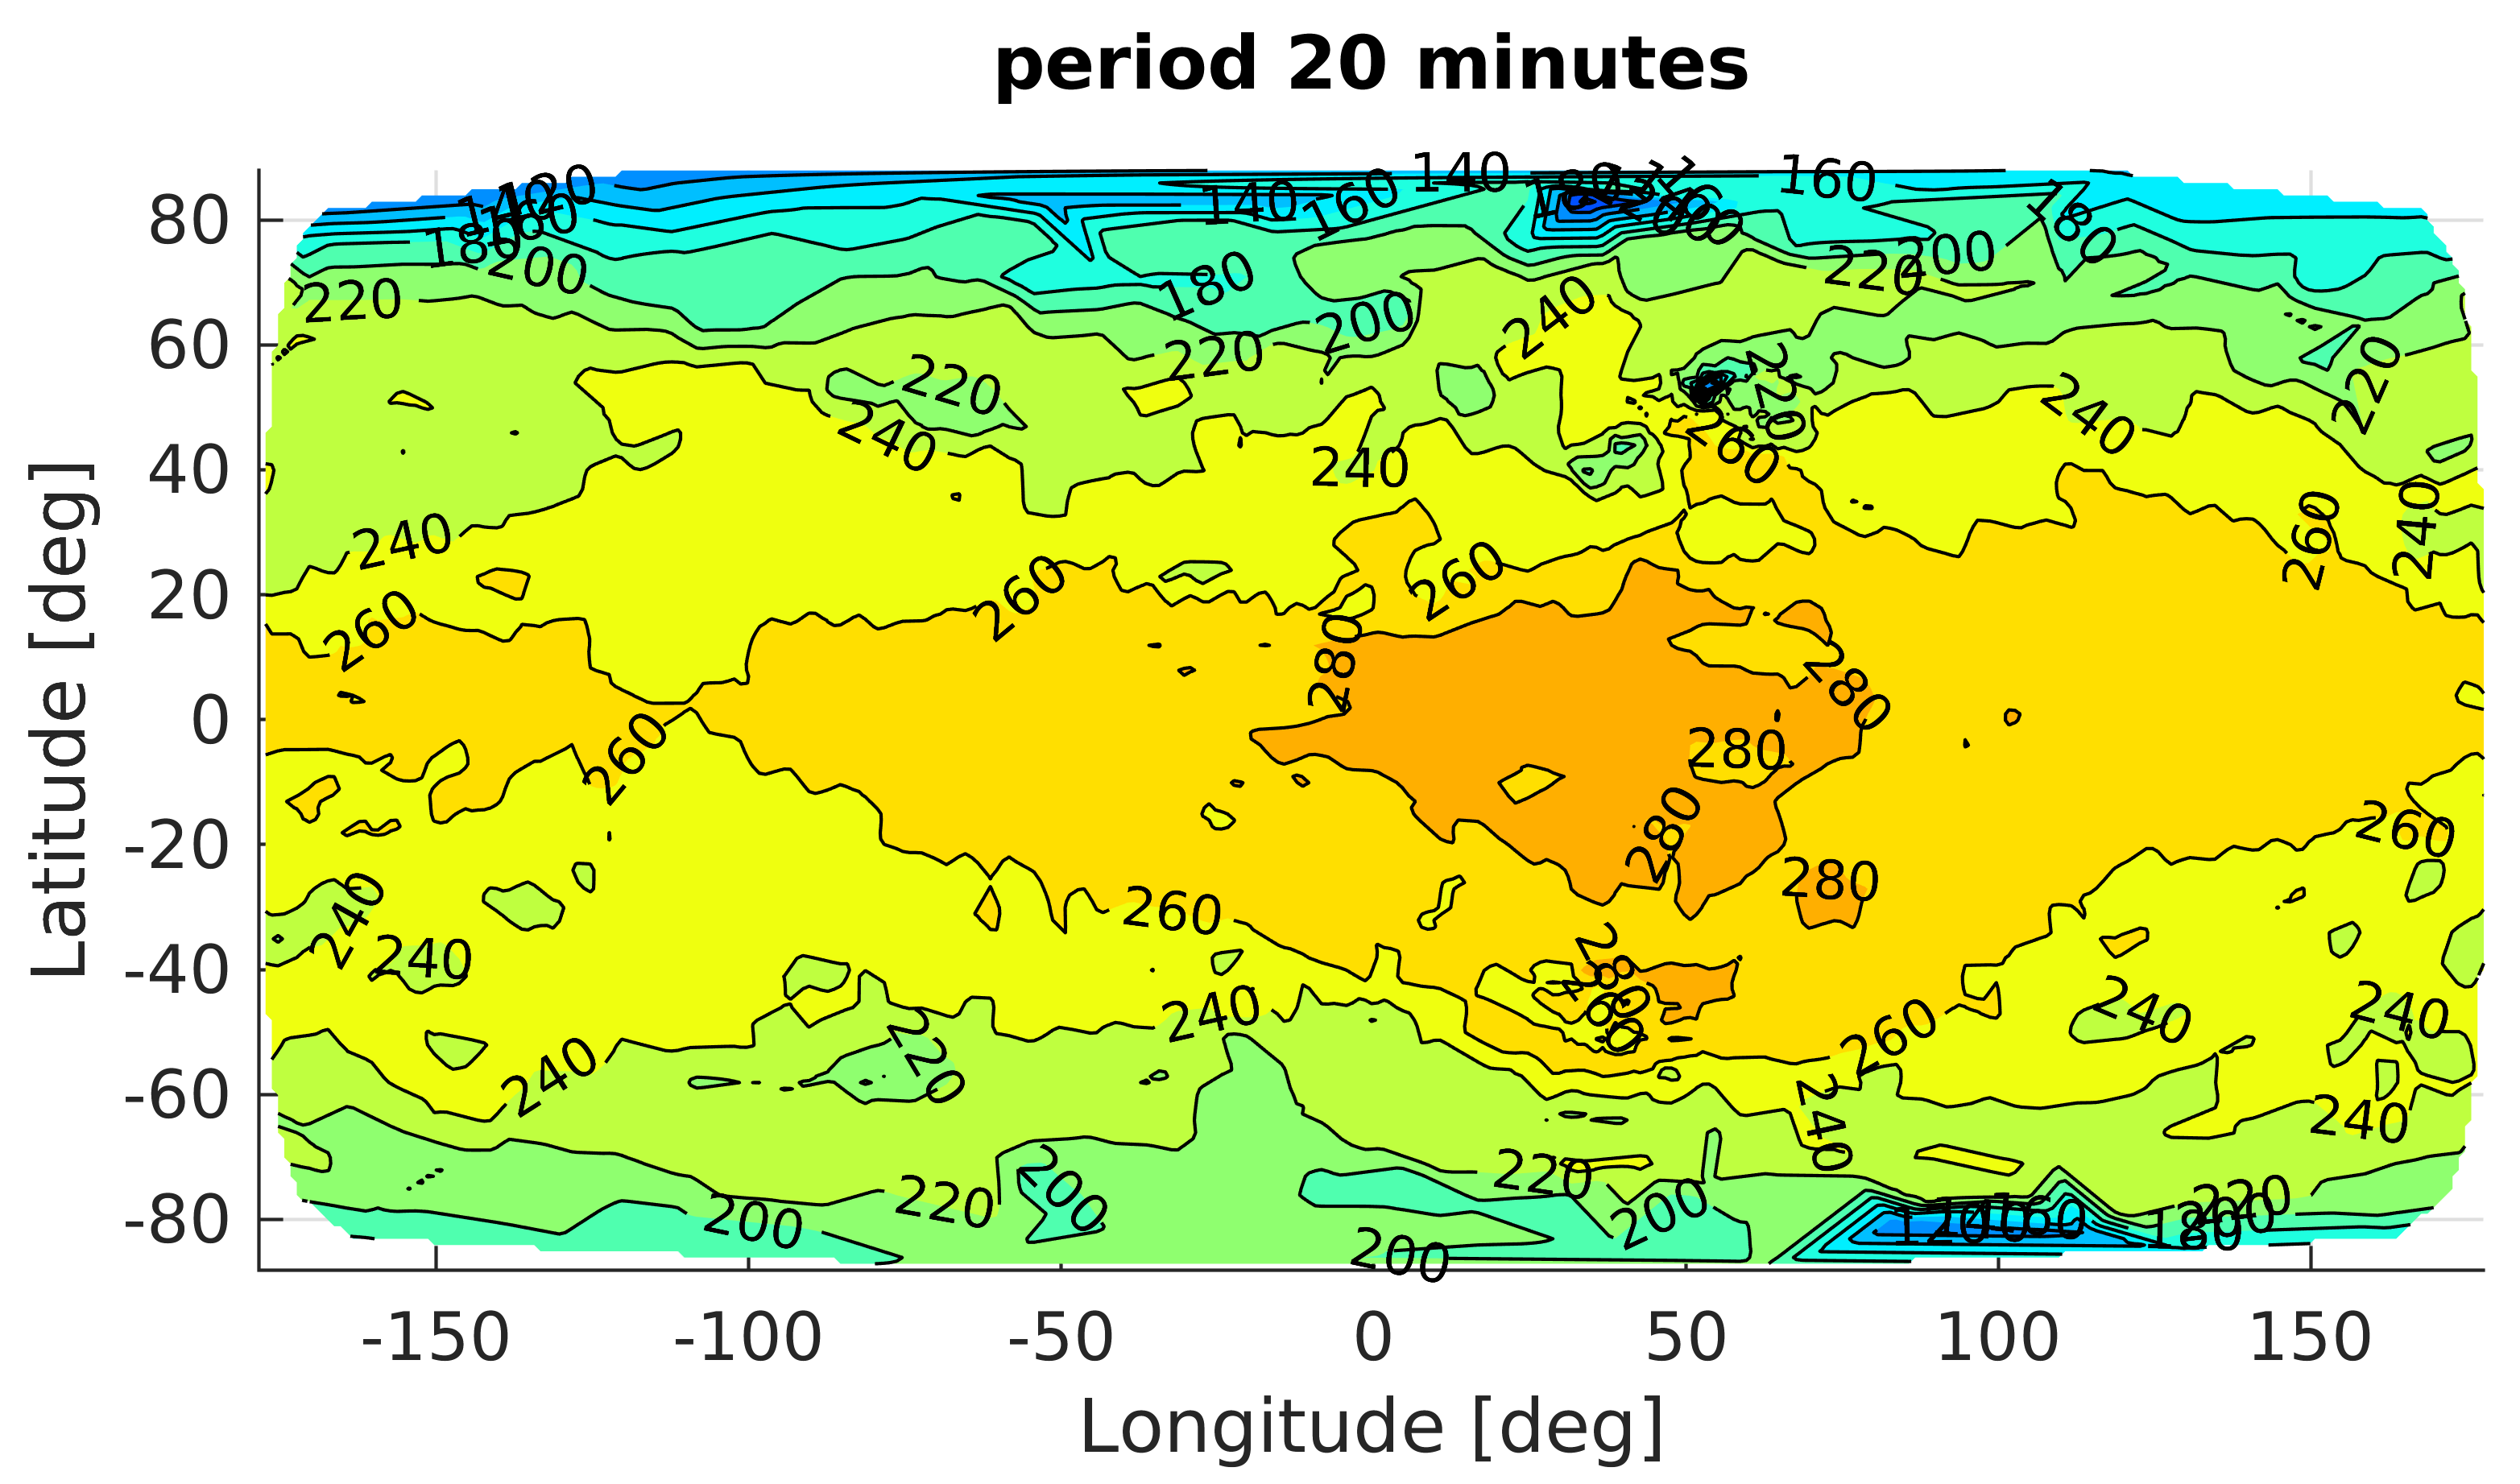
\includegraphics[width=\linewidth]{rsc/theo20mn.png}
    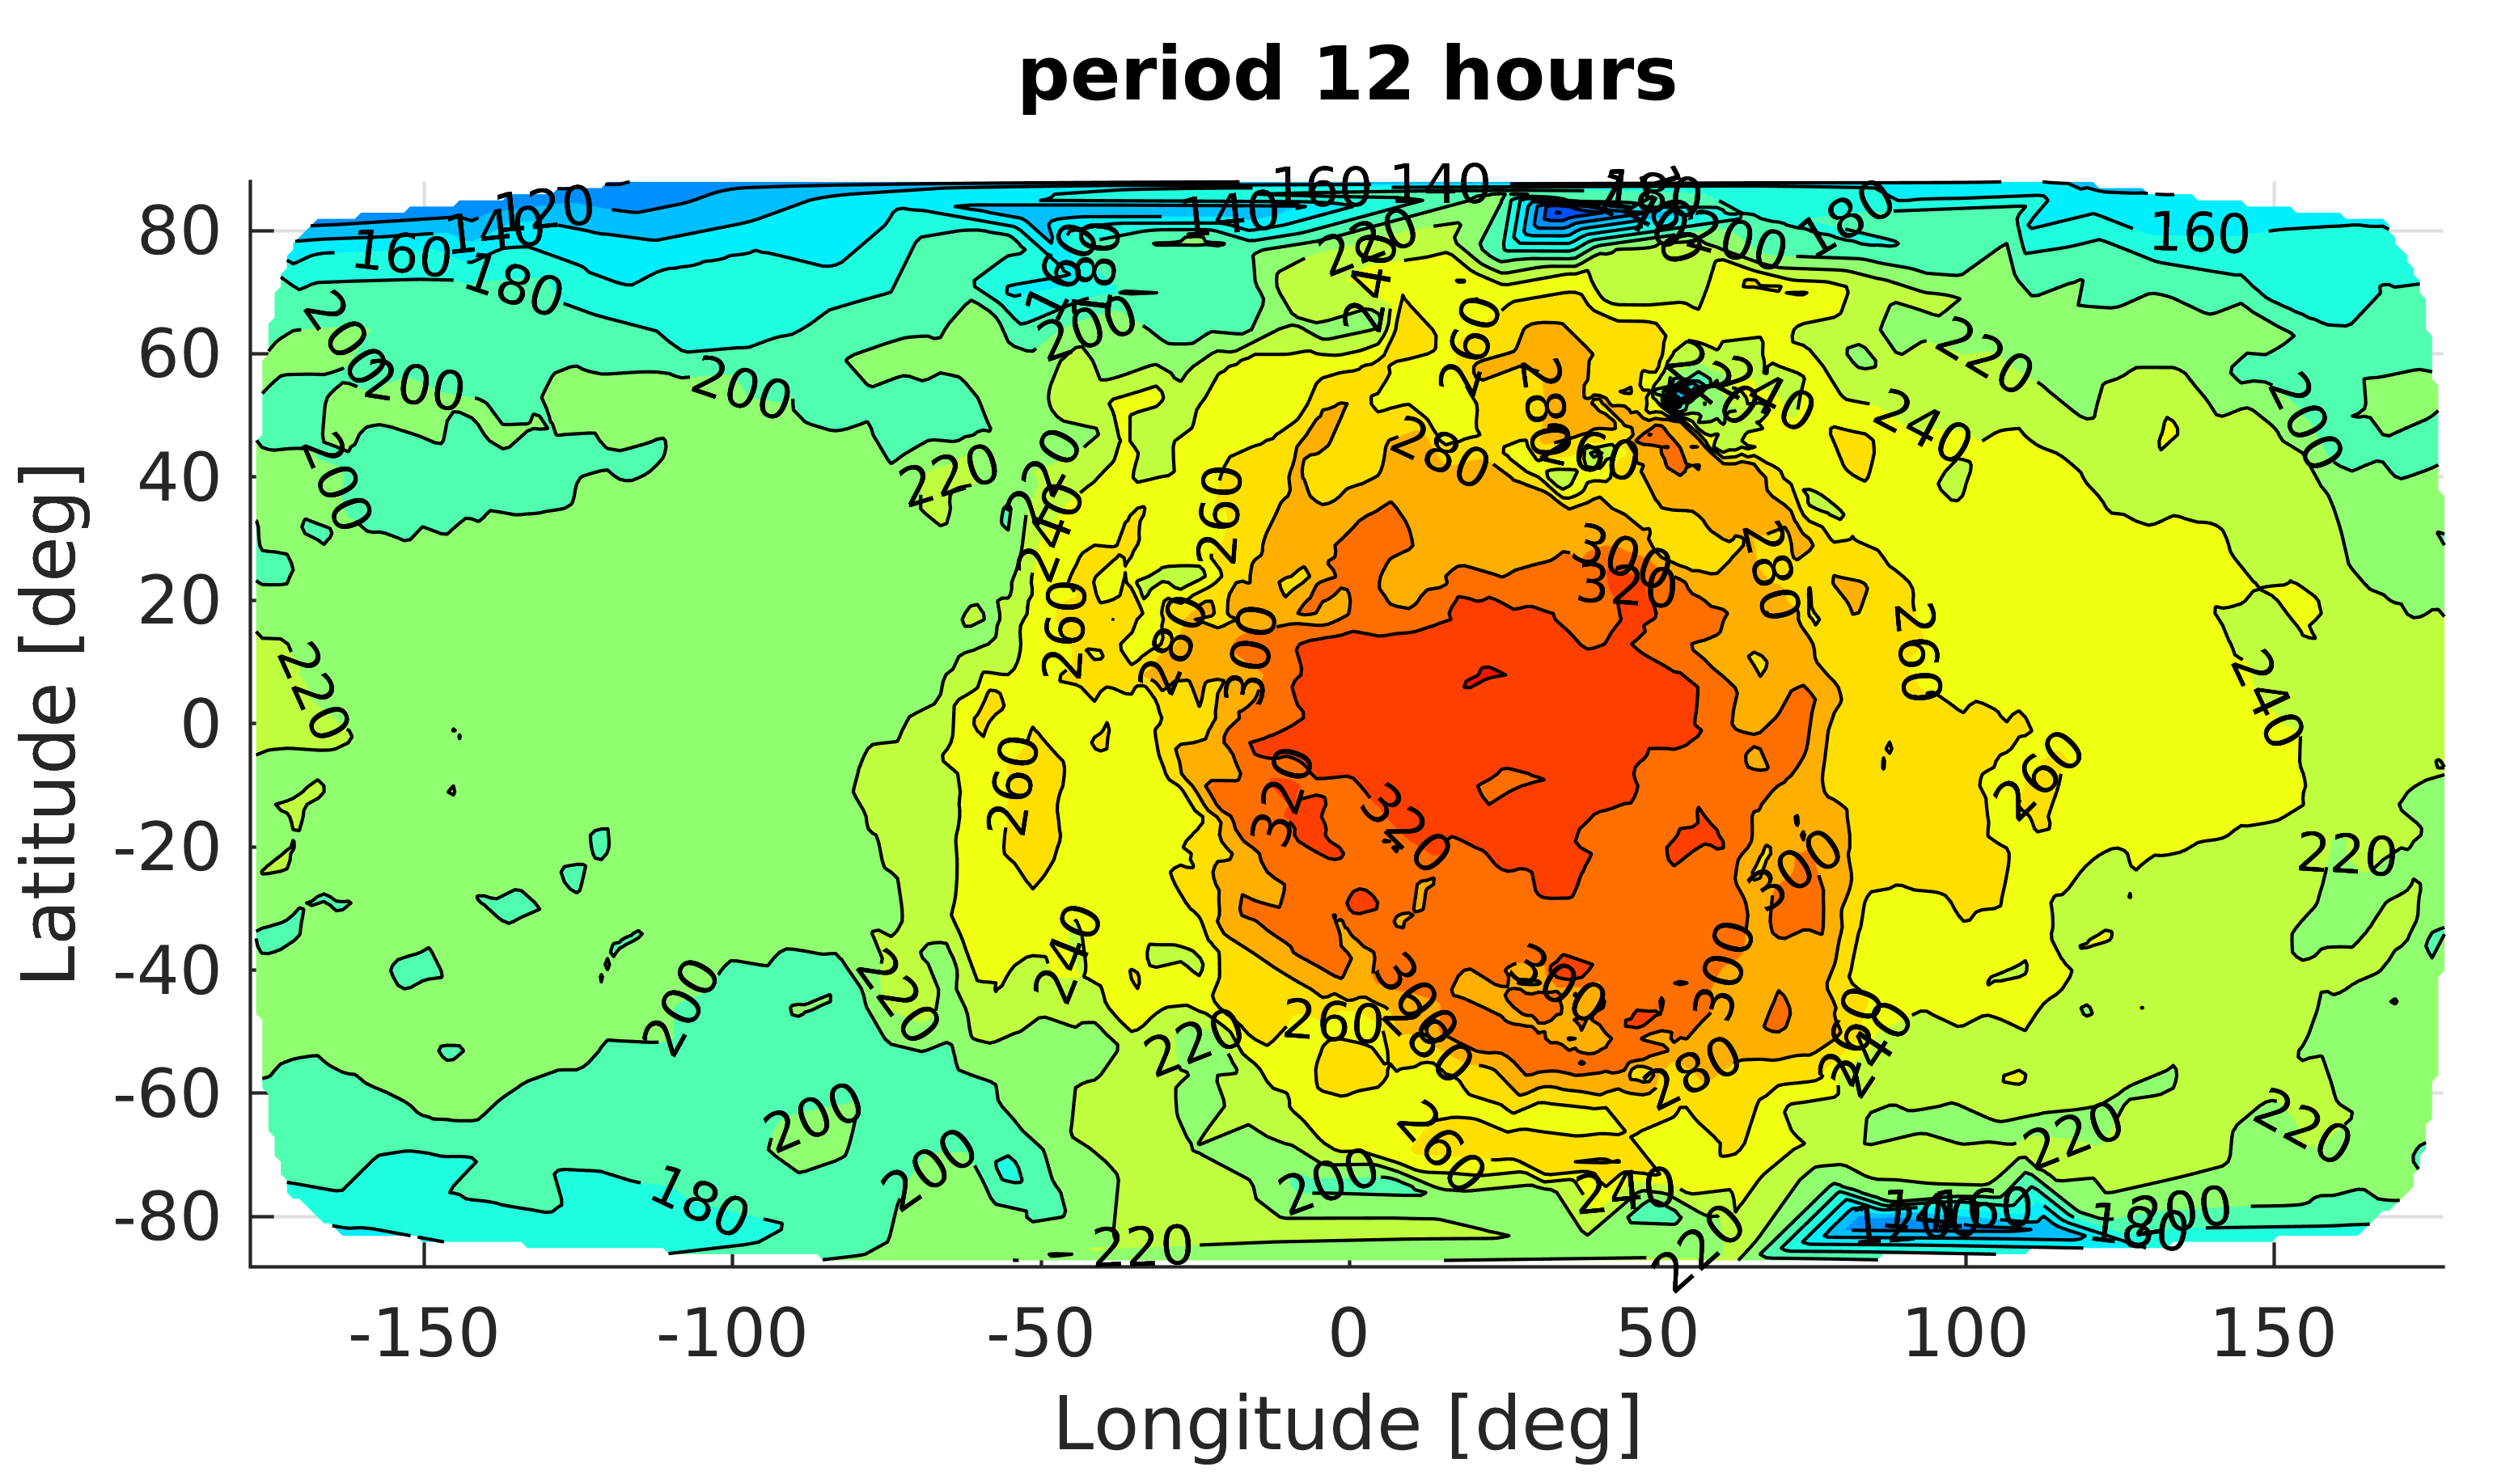
\includegraphics[width=\linewidth]{rsc/theo12h.png}
    \captionof{figure}{The first three images represent the asteroid with an orbital period fixed as $p_{orbital}=20$ minutes and a $\Gamma=500$, on the second line the other three images show an orbital period fixed as $p_{orbital}=12$ hours and a $\Gamma=500$}
\end{center}

We will see how the speed has impact the values, the difference speed gives us an overview on how it works.

The most differences between this figures are the mid day temperature is higher with a faster rotation.Temperatures around mid day are much more stable on the axis of rotation with a delta of 20 degrees variation while for a period of 12 hours temperatures are colder around the mid day area.\\[10pt]

More faster the asteroid his, higher are the temperature on a dedicate point. It's due that the rotation show to the sun more often their surfaces so they have higher temperature.
When the asteroid is slower we see that only the obliquity axis have hight temperature. We have created our model as we have presented before. \\[10pt]
To go through, we will look on why the thermal model map change.\\ [10pt]
When the asteroid is faster the pole on the obliquity axis stay more often on the view of the sun, it make that the temperature is higher on that point and colder on the extreme point.\\ [10pt]
When the asteroid is slower the temperature is distributed more uniformly over the whole of the asteroid, which means that we will find fairly hot temperatures on the skew axis but also cooler temperatures over the rest of the asteroid.\\[11pt]

We can apply a thermal map of her shap model using SMBT, using the value from Matlab it show us a 3D map.\\[10pt]

\begin{center}
	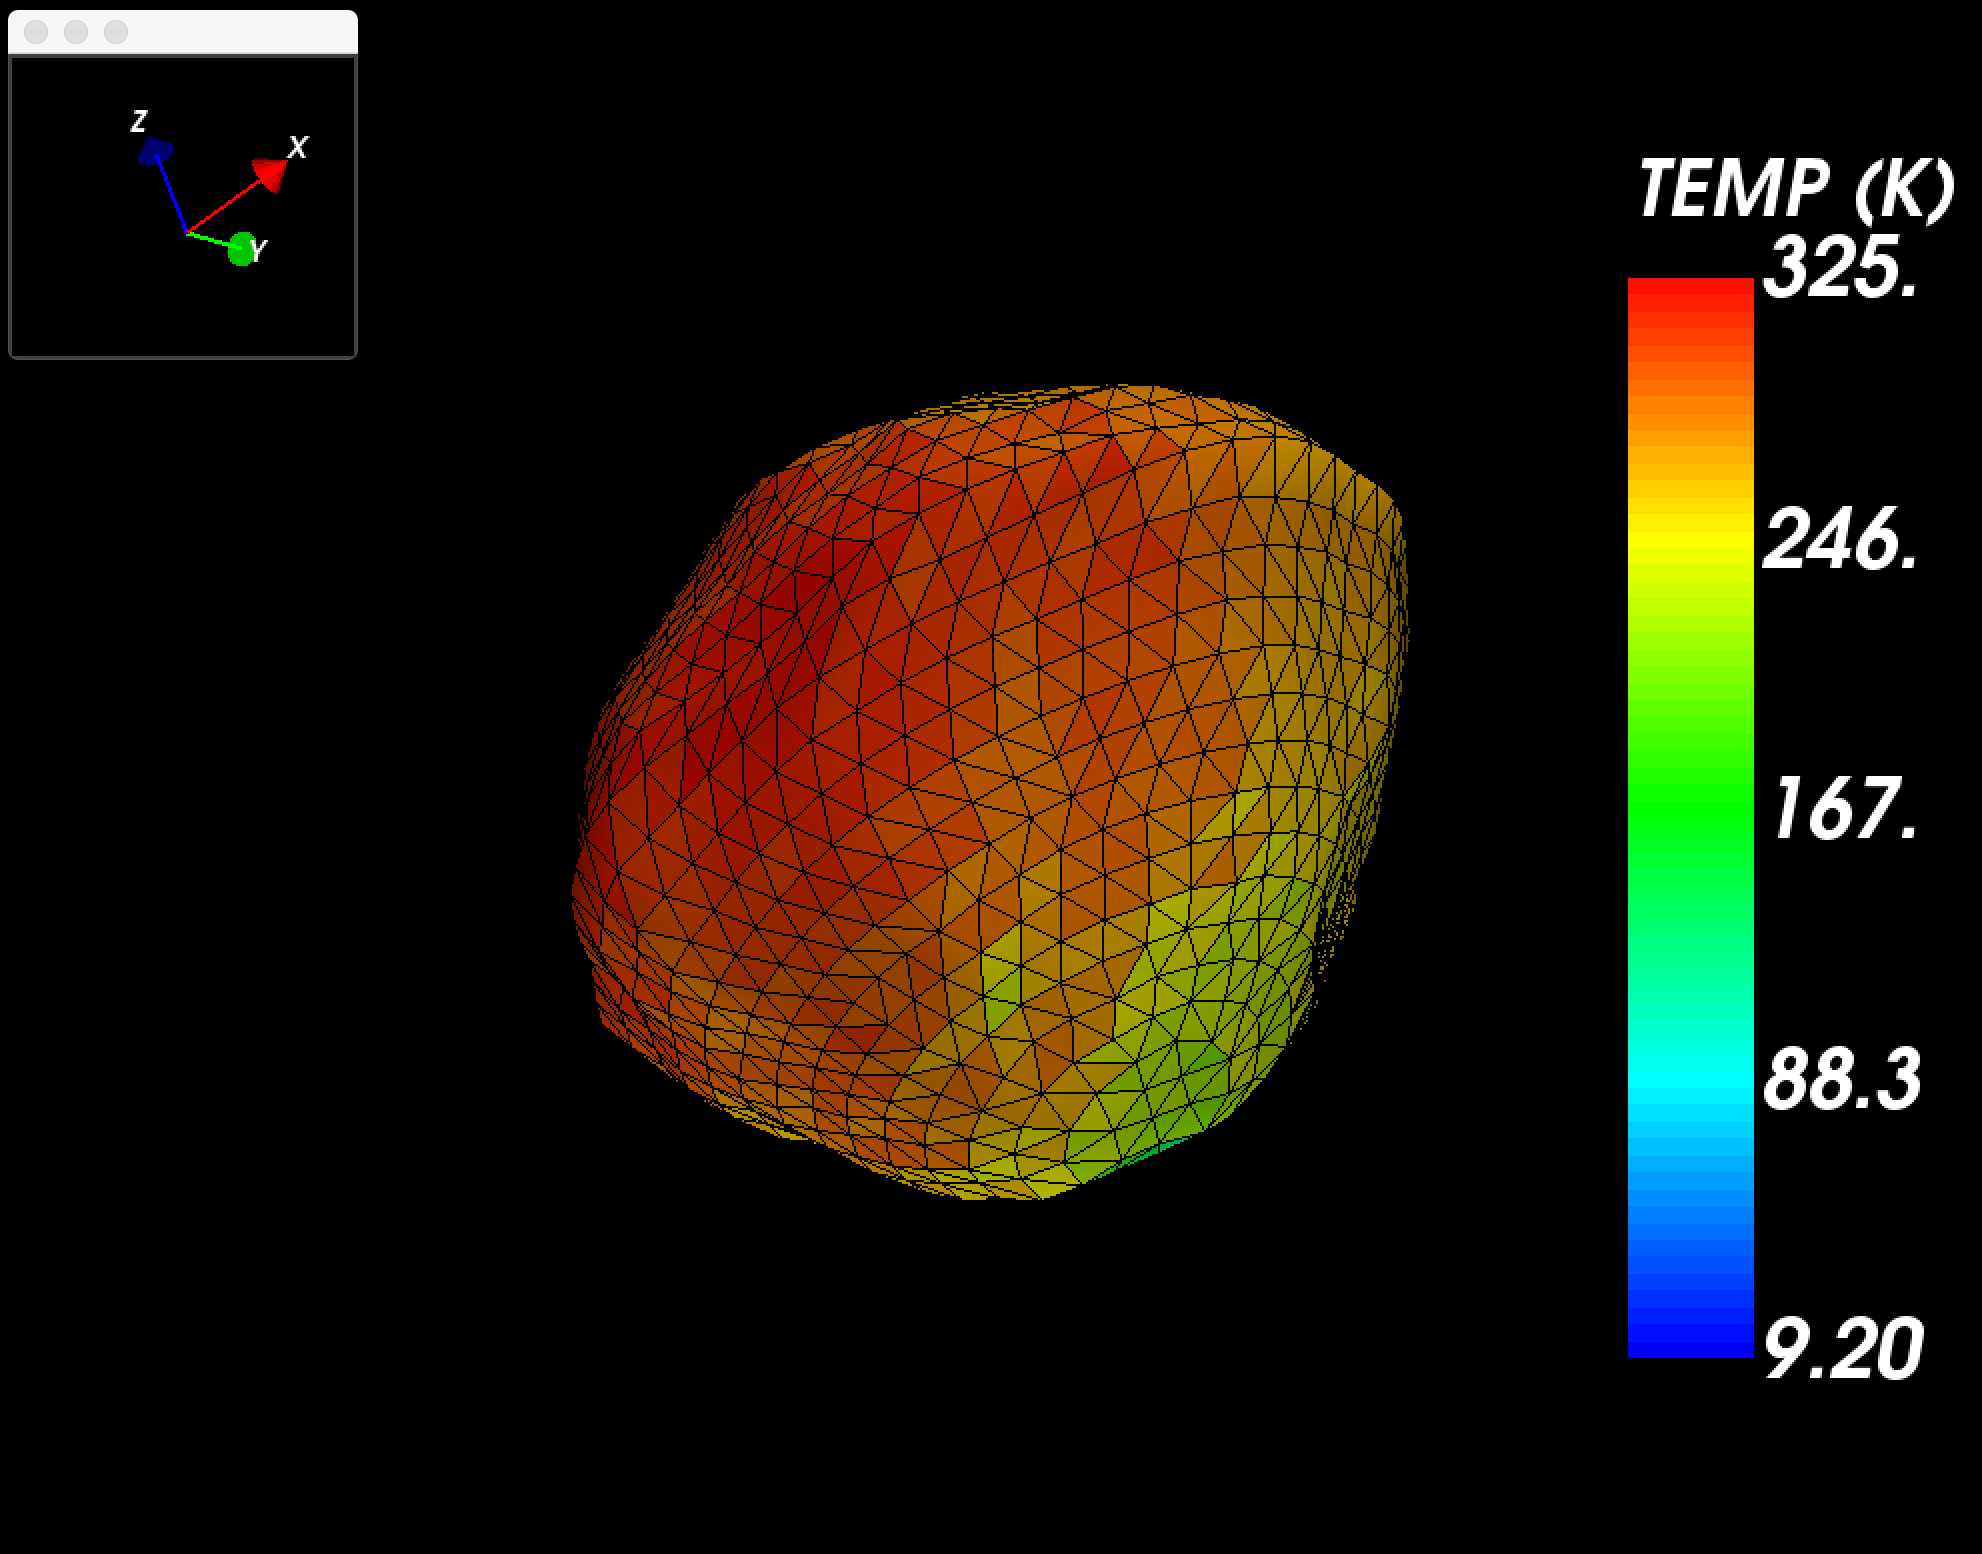
\includegraphics[width=\linewidth]{rsc/HO3_3D_normalspeed}
	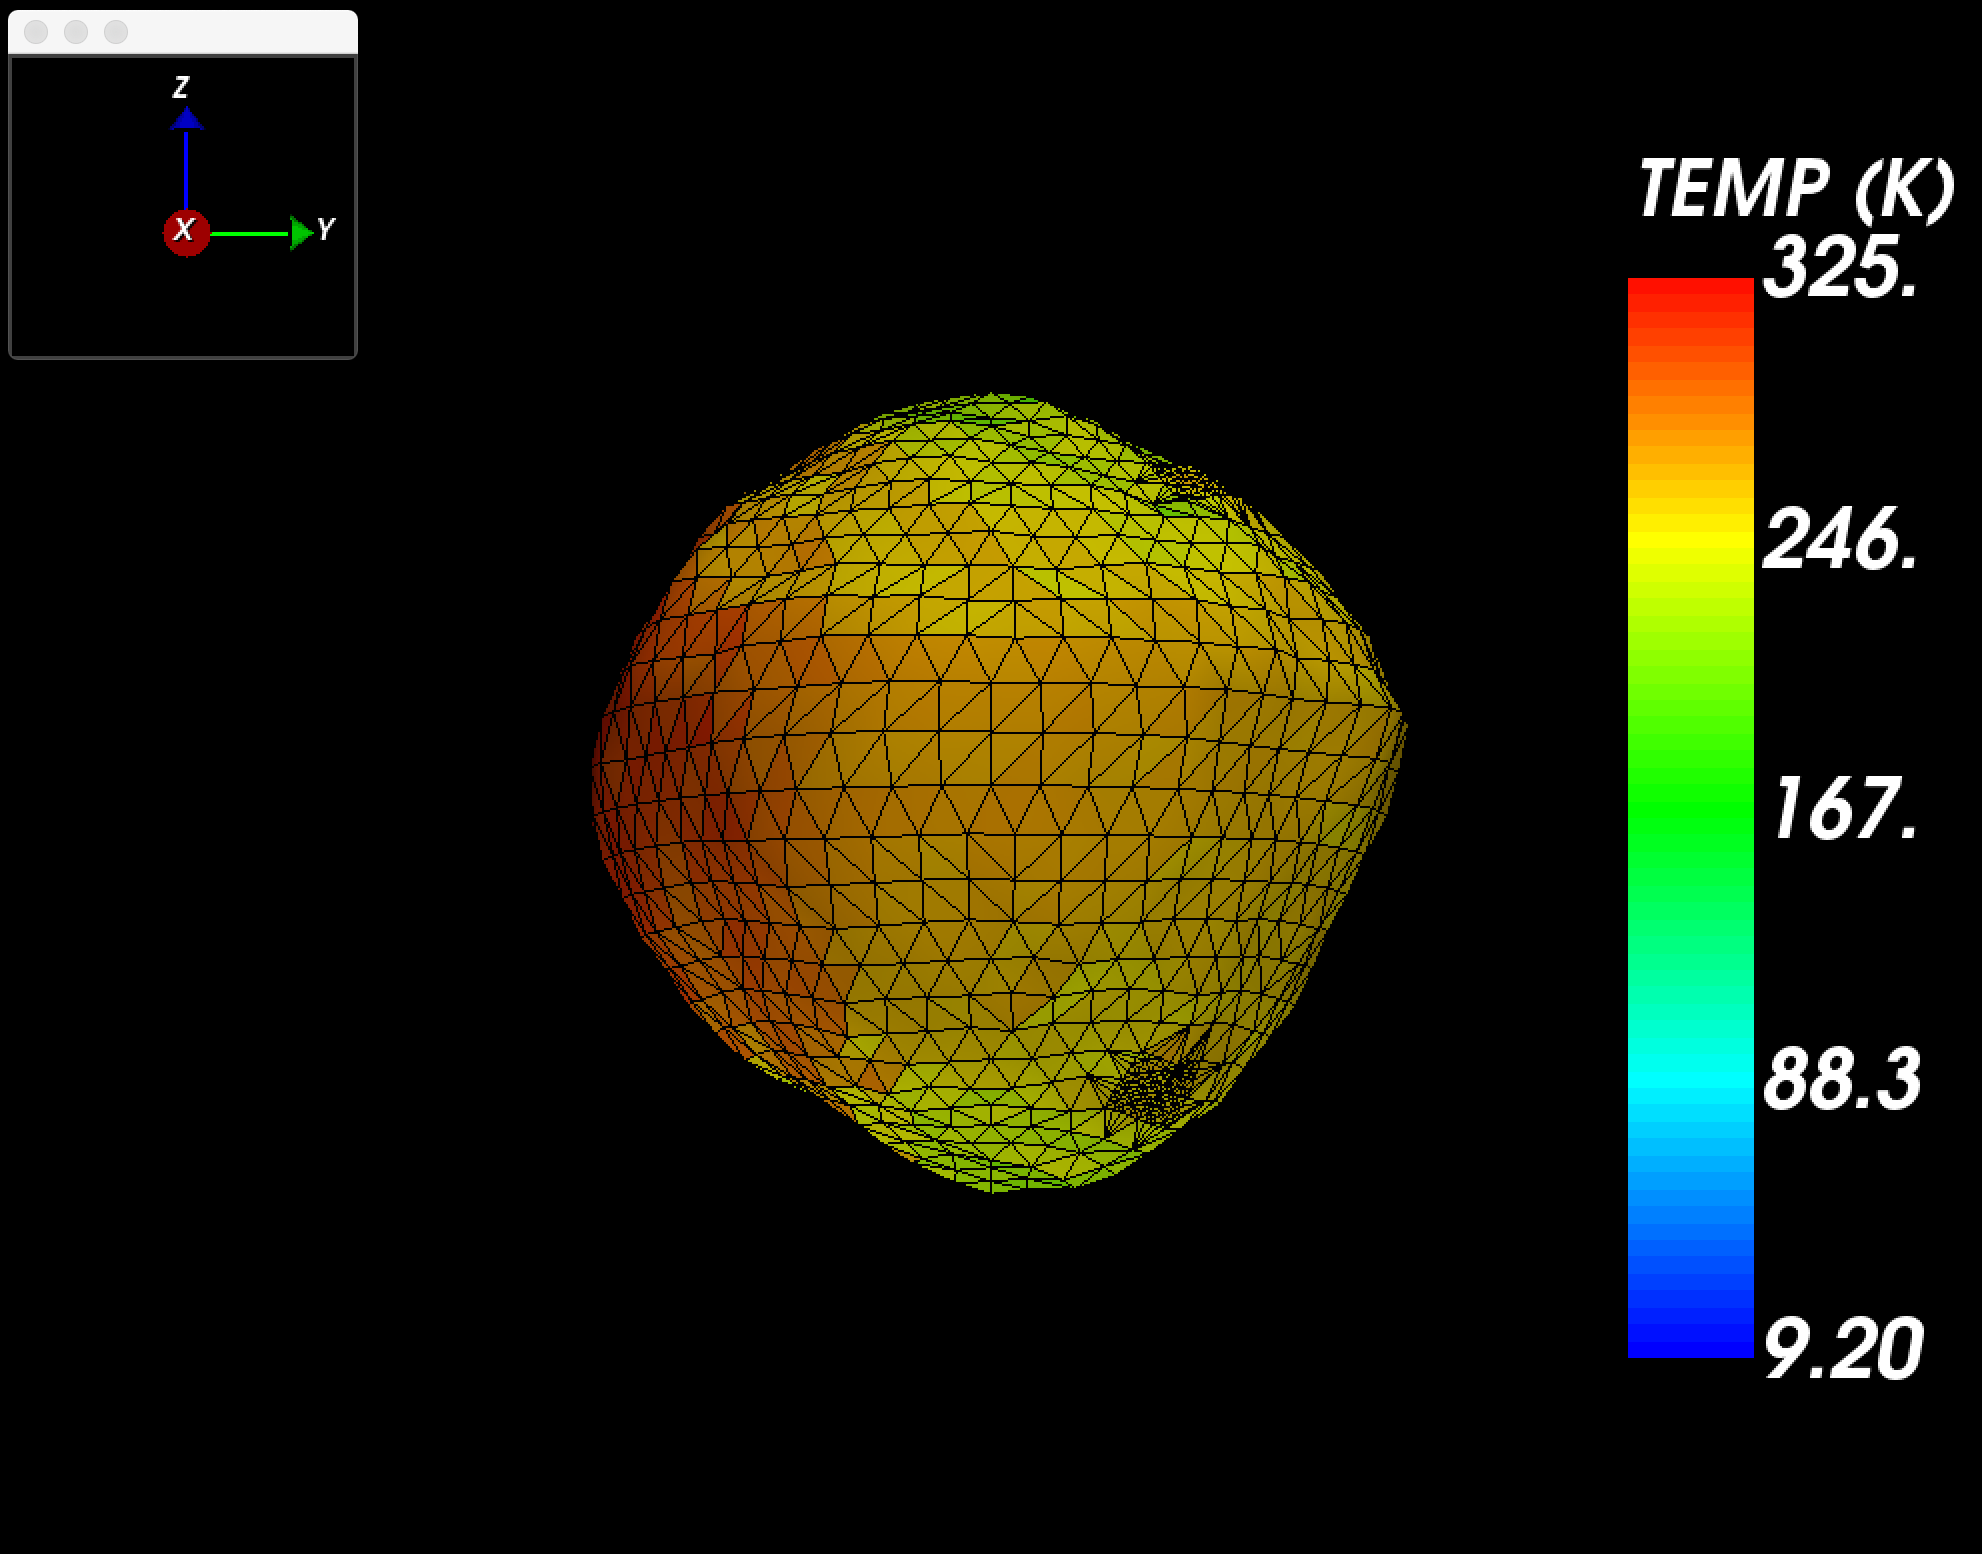
\includegraphics[width=\linewidth]{rsc/HO3_Xaxis_normalspeed}
	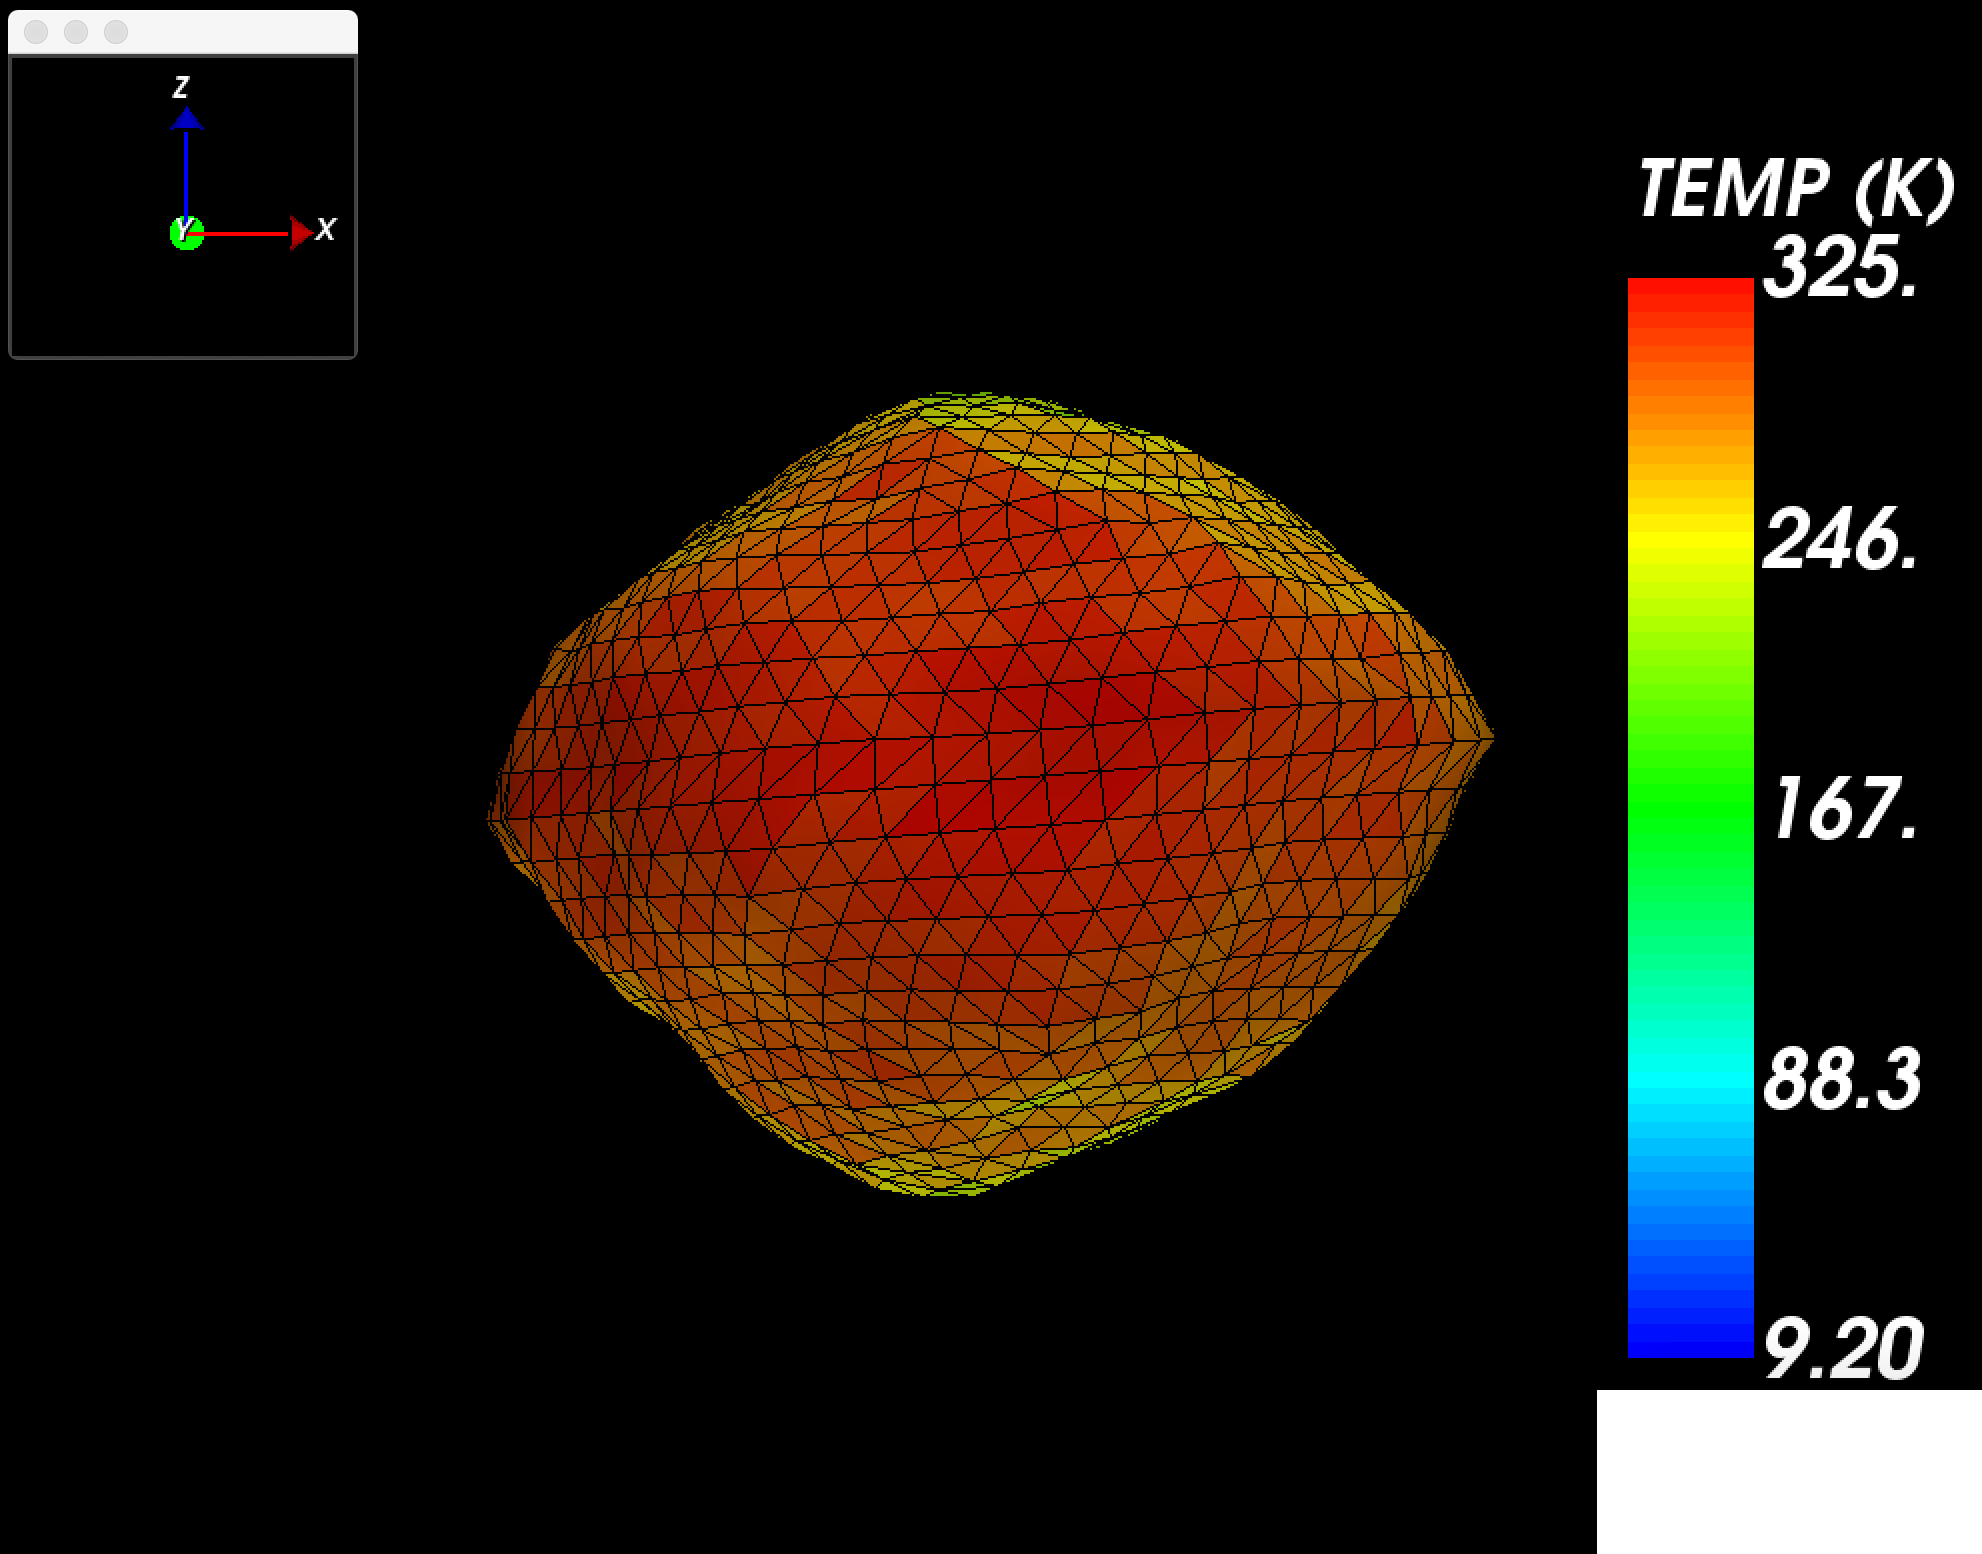
\includegraphics[width=\linewidth]{rsc/HO3_Yaxis_normalspeed}
	\captionof{figure}{3D thermal model}
\end{center}

